\section{Appendix: SCV Syntax, Specifications, Experimental Results, and Formal Definitions}
\label{sec:appendix}
%\subsection{SCV: Syntax}
\begin{lstlisting}[float=tp,captionpos=b,caption={Smart contract property specification for a simple contract},label={lst:smart-contract-property-specification},numbers=left]
mcontract name = spec
  code := {...}
  input := t
  output := t'
  pre-condition := p
  post-condition := p'
\end{lstlisting}

\begin{lstlisting}[float,captionpos=b,caption={Multiple entrypoint specification syntax (option 1)},label={lst:multiple-entrypoint-specification-1},numbers=left][h]
mcontract name = spec
   entrypoint %a 
      code := {c1}
      input := t1
      output := t1'
      pre-condition := p1
      post-condition := p1'
   entrypoint %b 
      ...
   <entrypoint relations>
\end{lstlisting}

\begin{lstlisting}[float,captionpos=b,caption={Multiple entrypoint specification syntax (option 2)},label={lst:multiple-entrypoint-specification-2},numbers=left][h]
mcontract name = spec
   storage := t1
   entrypoint %a 
      code := {c1}
      parameter := t2
      pre-condition := p1
      post-condition := p1'
   entrypoint %b 
      ...
   <entrypoint relations>
\end{lstlisting}

%\subsection{The Auction contract}
\begin{lstlisting}[float=tp,captionpos=b,caption={Auction contract specification},label={lst:auction-contract-specification},numbers=left]
mcontract auction = spec 
  storage := Pair (auction_open: bool) 
                   Pair (highest_bidder: address)
                        (contract_owner: address))
  entrypoint %bid
    code := {CDR; UNPAIR; DUP; IF {} {PUSH string 'already
     closed'; FAILWITH}; SWAP; UNPAIR; BALANCE; AMOUNT; 
     AMOUNT; ADD; COMPARE; GT; IF {} {PUSH string 'not 
     higher than the current highest bid'; FAILWITH};
     CONTRACT unit; IF_NONE {PUSH string 'invalid highest 
     bidder address'; FAILWITH} {}; AMOUNT; BALANCE; SUB; 
     IF_NONE {FAILWITH} {}; PUSH unit Unit; TRANSFER_TOKENS; 
     NIL operation; SWAP; CONS; DIP {SWAP; 
     DIP {SENDER; PAIR}; PAIR}; PAIR}
    parameter := Unit 
    pre-condition := auction_open = true
       && Amount > pre_Balance
       && get_contract (unit, highest_bidder) = 
          Some (c: contract unit)
    post-condition := auction_open = true
       && post_highest_bidder = Sender 
       && post_contract_owner = contract_owner 
       && post_Balance = Amount 
       && transfer_token (Unit, pre_Balance, c);
  entrypoint %close
    code := {CDR; UNPAIR; IF {}{PUSH string 'already closed'; 
     FAILWITH}; DUP; CDR; DUP; SENDER; COMPARE; EQ;
     IF {} {PUSH string 'not owner'; FAILWITH};
     DIP {PUSH bool false; PAIR}; CONTRACT unit; 
     IF_NONE {PUSH string 'invalid address'; FAILWITH} {} ;
     BALANCE; PUSH unit Unit; TRANSFER_TOKENS; 
     NIL operation; SWAP; CONS; PAIR}
    parameter := Unit
    pre-condition := auction_open = true
       && Sender = contract_owner  
       && get_contract (unit, contract_owner) = 
          Some (c: contract unit)              
    post-condition := post_auction_open  = false
       && post_Balance = 0 
       && transfer_token (Unit, pre_Balance + Amount, c) 
  (%create -> %bid) with (auction_open = true)  
       && (Amount > pre_Balance) 
       && get_contract (unit, highest_bidder) = 
           Some (c: contract unit)
  | (%create  -> %close) with (auction_open = true) 
       && (Sender = contract_owner)
       && get_contract (unit, contract_owner) = 
          Some (c: contract unit)
  | (%bid -> %bid) with (Amount > pre_Balance) 
       && get_contract (unit, highest_bidder) = 
          Some (c: contract unit)
  | (%bid -> %close) with (Sender = contract_owner) 
       && get_contract (unit, contract_owner) = 
            Some (c: contract unit)
  | not (%close -> %bid)
  | not (%close -> %close)
\end{lstlisting}

\begin{lstlisting}[float=tp,captionpos=b,caption={Fail condition for auction contract bid entrypoint},label={lst:fail-condition-auction-contract-bid},numbers=left]
1. not (auction_open = true): 'Already closed'
2. (auction_open = true) && not (Amount > pre_Balance):
   'Not higher than the current highest bid'
3. (auction_open = true) && (Amount > pre_Balance) && 
   get_contract (unit, highest_bidder) = None:
   'Invalid highest bidder address' 
\end{lstlisting}

\begin{lstlisting}[float=tp,captionpos=b,caption={Fail condition for auction contract close entrypoint},label={lst:fail-condition-auction-contract-close},numbers=left]
1. not (auction_open = true): 'Already closed'
2. (auction_open = true) && not (Sender = contract_owner): 
    'Not the owner'
3. (auction_open = true) && (Sender = contract_owner) &&
   get_contract (unit, contract_owner) = None:
  'Invalid contract owner address'
\end{lstlisting}
%\subsection{The USDtz contract}
\begin{lstlisting}[float=tp,captionpos=b,caption={Storage of the USDtz smart contract},label={lst:storage-udstz-contract}]
(pair
  (big_map %ledger
    (address :user)
    (pair (nat :balance)
          (map :approvals (address :spender) (nat :value))))
  (pair (address %admin)
        (pair (bool %paused) (nat %totalSupply))))
\end{lstlisting}
\begin{lstlisting}[float,captionpos=b,caption={Fail conditions for the \lstinline/transfer/ entrypoint},label={lst:transfer-udstz-contract},numbers=left]
1. (paused = true): 'TokenOperationsArePaused'
2. not (paused = true) 
   && get_big_map (from, ledger) = None : 'NotEnoughBalance'
3. not (paused = true) 
   && get_big_map (from, ledger) = Some sbvar 
   && sbvar = Pair sbvar1 sbvar2 
   && not (sbvar1 >= value) : 'NotEnoughBalance'
4. not (paused = true) 
   && get_big_map (from, ledger) = Some sbvar 
   && sbvar = Pair sbvar1 sbvar2 
   && get_map (Sender, sbvar2) = None: 'NotEnoughAllowance'
5. not (paused = true) 
   && get_big_map (from, ledger) = Some sbvar 
   && sbvar = Pair sbvar1 sbvar2 
   && get_map (Sender, sbvar2) = Some sbvar3 
   && sbvar1 >= value 
   && not (sbvar3 >= value): 'NotEnoughAllowance'
\end{lstlisting}

\begin{lstlisting}[float,captionpos=b,caption={Specification of the \lstinline/transfer/ entrypoint},label={lst:specification-transfer},numbers=left]
mcontract usdtz = spec 
 storage :=  Pair (ledger: big_map address 
  (pair nat (map address nat))) 
  (Pair (admin: address) 
          (Pair (paused: bool) (total_supply: nat)))
 entrypoint %transfer
   parameter := Pair (from: address)
         (Pair (to: address) (value: nat))
   pre-condition := not (paused  = true)
     && get_big_map (from, ledger) = 
       Some (v: pair nat (map address nat))
     && v = Pair (n: nat) (m: map address nat)
     && get_map (Sender, m) = Some (k: nat) 
     && (n >= value) && (k >= value)
   post-condition := get_big_map (from, post_ledger) = 
     Some (post_v:  pair nat (map address nat))
     && post_v = Pair (post_n: nat) (post_m: map address nat) 
     && get_map (Sender, post_m) = Some (post_k: nat) 
     && (post_n = n - value) && (post_k = k - value)
\end{lstlisting}

\begin{lstlisting}[float=tp,captionpos=b,caption={Fail conditions for the \lstinline/approve/ entrypoint},label={lst:approve-udstz-contract},numbers=left]
1. (paused = true): 'TokenOperationsArePaused'
2. not (paused = true) 
   && get_big_map (Sender, ledger) = Some sbvar 
   && sbvar = Pair sbvar1 sbvar2 
   && get_map (spender, sbvar2) = Some sbvar3 
   && not (value = 0) 
   && not (sbvar3 = 0): 'UnsafeAllowanceChange'
\end{lstlisting}
\begin{lstlisting}[float=tp,captionpos=b,caption={Specification of the \lstinline/approve/ entrypoint (Property 1)},label={lst:specification-approve-1},numbers=left]
entrpoint %approve
   parameter := Pair (spender: address) (value: nat)
   pre-condition := not (paused = true)
      && get_big_map (Sender, ledger) = 
        Some (v: pair nat (map address nat))
      && v = Pair (n: nat) (m: map address nat) 
      && get_map (spender, m) = Some (k: nat) 
      && not (k = 0) && (value = 0)
   post-condition := get_big_map (Sender, post_ledger) = 
        Some (post_v:  (pair nat (map address nat))
      && post_v = Pair (post_n: nat) (post_m: map address nat) 
      && get_map (spender, post_m) = Some (post_k: nat) 
      && (post_k = 0) ;
\end{lstlisting}
\begin{lstlisting}[float=tp,captionpos=b,caption={Specification of the \lstinline/approve/ entrypoint (Property 2)},label={lst:specification-approve-2},numbers=left]
   pre-condition := not (paused = true) 
      && get_big_map (Sender, ledger) = 
        Some (v: option (pair nat (map address nat))) 
      && v = Pair (n: nat) (m: map address nat) 
      && get_map (spender, m) = Some (k: nat) 
      && (k = 0) && not (value = 0)
   post-condition := get_big_map (Sender, post_ledger) = 
        Some (post_v: option (pair nat (map address nat))) 
      && post_v = Pair (post_n: nat) (post_m: map address nat) 
      && get_map (spender, post_m) = Some (post_k: nat) 
      && (post_k = value) ;
\end{lstlisting}
\begin{lstlisting}[float=tp,captionpos=b,caption={Specification of the \lstinline/getBalance/ entrypoint},label={lst:specification-get-balance},numbers=left]
entrypoint %getBalance
   parameter := Pair (owner: address) (c: contract nat)
   pre-condition :=  get_big_map (owner, ledger) = 
        Some v: option (pair nat (map address nat)) 
      && v  = Pair (k: nat) (m: (map address nat))
   post-condition := post_ledger = ledger 
      && post_admin = admin 
      && post_paused = paused 
      && post_total_supply = total_supply 
      && post_Balance = pre_Balance 
      && transfer_token (k, Amount, c) ;

   pre-condition :=  get_big_map (owner, ledger) = 
        None option (pair nat (map address nat)) 
   post-condition := post_ledger = ledger 
      && post_admin = admin 
      && post_paused = paused 
      && post_total_supply = total_supply 
      && post_Balance = pre_Balance 
      && transfer_token (0, Amount, c) ;
\end{lstlisting}
%\subsection{The Kolibri Oracle contract}

\begin{lstlisting}[float,captionpos=b,caption={Kolibri oracle contract},label={lst:kolibri-oracle-contract},numbers=left]
parameter
 (or
   (or (unit %default) (contract nat %getXtzUsdRate))
   (or
     (pair string (pair timestamp nat) %getXtzUsdRate_callback)
     (or
       (address %setGovernorContract) 
       (nat %setMaxDataDelaySec)))) ;
storage
 (pair
   (pair (option %clientCallback address) 
         (address %governorContractAddress))
   (pair (address %harbingerContractAddress) 
         (pair (nat %maxDataDelaySec) (int %state)))) ;
\end{lstlisting}

\begin{figure}[tp]
    \centering
    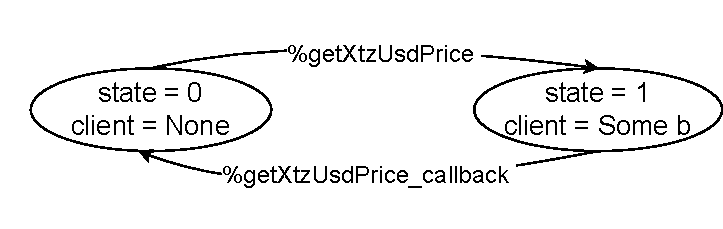
\includegraphics[width=0.8\textwidth]{kolibri(1)}
    \caption{Kolibri oracle entrypoint relations}
    \label{fig:kolibri-oracle-emtrypoint-relations}
\end{figure}
\begin{lstlisting}[float=tp,captionpos=b,caption={Kolibri oracle contract specification},label={lst:kolibri-contract-specification},numbers=left]
mcontract kolibri = spec 
  storage := (Pair (Pair (client: option address) 
     (governor: address))
     (Pair (harbinger: address) 
           (Pair (maxDelay: nat) (state: int))))
  entrypoint %getXtzUsdRate
    code := {...}
    parameter := (ct : contract nat) 
    pre-condition := (Amount = 0) && (state = 0)
    get_contract (pair string (contract pair 
    string (pair timestamp nat)), harbinger) = Some c
    post-condition := post_state = 1
       && client = Some (b: address) ;
  entrypoint %getXtzUsdRate_callback
    code := {...}
    parameter := Pair (s: string) 
       (Pair (t: timestamp) (n: nat))
    pre-condition :=  state = 1 
       && Sender = harbinger  
       && s = 'XTZ-USD' 
       && Now - t < maxDelay 
       && Now - t >= 0 
       && client = Some a 
       && get_contract (nat, a) = Some c    
    post-condition := post_state = 0 
       && post_client = None 
       && transfer_token(n, 0, c) ;
  entrypoint %setGovernorContract
    code := {...}
    parameter := (gover : address) 
    pre-condition :=  (Sender = governor)                  
    post-condition := (post_governor = gover) 
       && (post_maxDelay = maxDelay) 
       && (post_harbinger = harbinger) ;
  entrypoint %setMaxDataDelaySec
    code := {...}
    parameter := (delay: nat)
    pre-condition := (Sender = governor)             
    post-condition := (post_maxDelay = delay) 
       && (post_client = client) 
       && (post_harbinger = harbinger) ;
  (%getXtzUsdRate -> %getXtzUsdRate_callback) with
     (Sender = harbinger)
     && (s = 'XTZ-USD') 
     && (Now - t >= 0)  
     && (Now - t < maxDelay)  
     && client = Some a 
     && get_contract (nat, a) = Some c    
  | (%getXtzUsdRate_callback  -> %getXtzUsdRate) with 
    (Amount = 0) 
    && get_contract (pair string (contract pair 
    string (pair timestamp nat)), harbinger) = Some c
  | not (%getXtzUsdRate -> %getXtzUsdRate) 
  | not (%getXtzUsdRate_callback -> %getXtzUsdRate_callback)
\end{lstlisting}
\begin{lstlisting}[float=tp,captionpos=b,caption={Failwith condition for the entrypoint setXtzUsdPrice\_callback},label={lst:setXtzUsdPrice_callback},numbers=left]
1. not (state = 1): 12
2. (state = 1) && not (Sender = harbinger): 3
3. (state = 1) &&  (Sender = harbinger) 
&& not ('XTZUSD' = s): 14
4. (state = 1) &&  (Sender = harbinger) && ('XTZUSD' = s)
&& (Now - t >= 0) && not (Now - t < maxDelay): 17
5. (state = 1) &&  (Sender = harbinger) && ('XTZUSD' = s)
&& not (Now - t >= 0): Unit
6. (state = 1) &&  (Sender = harbinger) && ('XTZUSD' = s)
&& (Now - t >= 0) && (Now - t < maxDelay) 
&& (client = Some sbvar) 
&& get_contract (nat, sbvar) = None: Unit
7. (state = 1) &&  (Sender = harbinger) && ('XTZUSD' = s)
&& (Now - t >= 0) && (Now - t < maxDelay) 
&& (client = None): Unit
\end{lstlisting}

\begin{lstlisting}[float=tp,captionpos=b,caption={Failwith condition for the entrypoint setMaxDataDelaySec},label={lst:setMaxDataDelaySec},numbers=left]
not (Sender = governor): 4
\end{lstlisting}
\newpage
%\subsection{Formal Definitions}
%\label{sec:formal-definitions}
\begin{figure} []
\begin{align*}
T, U &::= \\
   &\Mid\ \langle \text{comparable type}\rangle \\
   &\Mid\ \text{option}\ \langle\text{type}\rangle \\
   &\Mid\ \text{list}\ \langle\text{type}\rangle \\
   &\Mid\ \text{set}\ \langle\text{comparable type}\rangle \\
   &\Mid\ \text{operation} \\
   &\Mid\ \text{contract}\ \langle\text{type}\rangle \\
   &\Mid\ \text{ticket}\ \langle\text{comparable type}\rangle \\
   &\Mid\ \text{pair}\ \langle\text{type}\rangle \langle\text{type}\rangle \\
   &\Mid\ \text{or}\ \langle\text{type}\rangle \langle\text{type}\rangle \\
   &\Mid\ \text{lambda}\ \langle\text{type}\rangle \langle\text{type}\rangle \\
   &\Mid\ \text{map}\ \langle\text{comparable type}\rangle \langle\text{type}\rangle \\
   &\Mid\ \text{big-map}\ \langle\text{comparable type}\rangle \langle\text{type}\rangle \\
   &\Mid\ \text{bls12-381-g1} \\
   &\Mid\ \text{bls12-381-g2} \\
   &\Mid\ \text{bls12-381-fr} \\
   &\Mid\ \text{sapling-transaction}\ \langle\text{natural number constant}\rangle \\
   &\Mid\ \text{sapling-state}\ \langle\text{natural number constant}\rangle \\
   &\Mid\ \text{chest} \\
   &\Mid\ \text{chest-key} \\
\langle\text{comparable type}\rangle ::= \\
   &\Mid\ \text{unit} \\
   &\Mid\ \text{never} \\
   &\Mid\ \text{bool} \\
   &\Mid\ \text{int}\\
   &\Mid\ \text{nat}\\
   &\Mid\ \text{string}\\
   &\Mid\ \text{chain-id}\\
   &\Mid\ \text{bytes}\\
   &\Mid\ \text{mutez}\\
   &\Mid\ \text{key-hash}\\
   &\Mid\ \text{key}\\
   &\Mid\ \text{signature}\\
   &\Mid\ \text{timestamp}\\
   &\Mid\ \text{address}\\
   &\Mid\ \text{tx-rollup-l2-address}\\
   &\Mid\ \text{option}\ \langle\text{comparable type}\rangle\\
   &\Mid\ \text{or}\ \langle\text{comparable type}\rangle \langle\text{comparable type}\rangle\\
   &\Mid\ \text{pair}\ \langle\text{comparable type}\rangle \langle\text{comparable type}\rangle \DOT \\
\end{align*}
\caption{Types}
\label{fig:type}
\end{figure}

\begin{figure}[h]
\begin{align*}
\text{t} &::= \\
   &\Mid\ \langle \text{variable} \rangle \\
   &\Mid\ \langle \text{account constant} \rangle \\
   &\Mid\ \langle \text{int constant} \rangle \\
   &\Mid\ \langle \text{string constant} \rangle \\
   &\Mid\ \langle \text{byte sequence constant} \rangle \\
   &\Mid\ \UNIT \\
   &\Mid\ \TRUE \\
   &\Mid\ \FALSE \\
   &\Mid\ \PAIR\ \text{t1 t2}\\
   &\Mid\ \LEFT\ \text{t}\\
   &\Mid\ \RIGHT\ \text{t}\\ 
   &\Mid\ \SOME\ \text{t}\\
   &\Mid\ \NONE \\
   &\Mid\ \text{\{t ; ... \}}\\
   &\Mid\ \text{\{ Elt t1 t2 ; ... \}}\\
   &\Mid\ \{ \langle\text{instruction}\rangle; ... \}   \\
\langle \text{variable} \rangle &::= \\ 
   &\Mid\ \VAR\\
\langle \text{account constant} \rangle &::= \\ 
   &\Mid\ \text{balance} \\
   &\Mid\ \text{amount} \\
   &\Mid\ \text{sender} \\
   &\Mid\ \text{source} \\
   &\Mid\ \text{now} \\
   &\Mid\ \text{level} \\
   &\Mid\ \text{chain-id} \\
   &\Mid\ \text{self}  \\
   &\Mid\ \text{self-address}  \\
   &\Mid\ \text{total-voting-power}  \\
   &\Mid\ \text{voting-power}  \\
\langle \text{natural number constant} \rangle &::= \\ 
   &\Mid\ \text {[0-9]+} \\
\langle \text{int constant} \rangle &::= \\
  &\Mid\ \langle \text{natural number constant} \rangle \\
  &\Mid\ \text{-} \langle \text{natural number constant} \rangle \\
\langle\text{string constant}\rangle &::= \\
  &\Mid\ \text{"} \langle \text{string content}\rangle\text{*"} \\
\langle\text{instruction}\rangle &::= \\
  &\Mid\ \DROP \\
  &\Mid\ \DROP \langle\text{natural number constant}\rangle \\
  &\text{...}
\end{align*}
\caption{Terms}
\label{fig:term}
\end{figure}



\subsubsection{Basic Instructions}

\paragraph{Control structures}
%EXE
\begin{mathpar}
  \inferrule[EXEC]
  {
    [\INSTRUCTIONONE, (\StackOne, \TYF) \STACKCONCAT \EMPTYSTACK, 
    Q]
    \StateTrans^*
    [ \EMPTYSTACK, (\StackOne', \TYS) \STACKCONCAT Q']
  }{
     [(\EXEC; \INSTRUCTION),   (\{\INSTRUCTIONONE\}, \TYF\ \rightarrow\ \TYS) \STACKCONCAT
    (\StackOne, \TYF) \STACKCONCAT \STACK, \PREDICATE \wedge Q] 
    \StateTrans \
    [ \INSTRUCTION, (\StackOne', \TYS) \STACKCONCAT \STACK,
    \PREDICATE \wedge Q']}
\end{mathpar}

%APPLY
\begin{mathpar}
  \inferrule[APPLY]
  {
  }{
    [(\APPLY; \INSTRUCTION), (\StackOne, \TYF) \STACKCONCAT(\{\INSTRUCTIONONE\}, \TLAMBDA\ (\TPAIR\ \TYF\  \TYS)\ \TYT) \STACKCONCAT\STACK, \PREDICATE] \StateTrans\\ [\INSTRUCTION, (\{\PUSH\ \TYF\ \StackOne; \IPAIR; \INSTRUCTIONONE\}, \TLAMBDA\ \TYS\ \TYT ) \STACKCONCAT\STACK, \PREDICATE]}
\end{mathpar}

%LAMBLA
\begin{mathpar}
  \inferrule[LAMBDA]
  {  
  }{
    [(\LAMBDA\ \TYF\ \TYS\ \{ \INSTRUCTIONONE \} ; \INSTRUCTION),\STACK, \PREDICATE] \StateTrans\ [\INSTRUCTION, (\{\INSTRUCTIONONE\}, \TLAMBDA\ \TYF\ \rightarrow\ \TYS) \STACKCONCAT\STACK, \PREDICATE]}
\end{mathpar}

\paragraph{Stack Manipulation}
%DIG
\begin{mathpar}
\inferrule[DIG]
  {
   \FLEN(\A) \EQ\ \N
  }
  {[(\DIG\ \N ; \INSTRUCTION), \A\ \At\ (\StackOne, \TY) \STACKCONCAT\B, \PREDICATE] \StateTrans 
[\INSTRUCTION, (\StackOne, \TY) \STACKCONCAT\A\ \At\ \B, \PREDICATE]}
\end{mathpar}

%DIP
\begin{mathpar}
  \inferrule[DIP]
  {
    [\INSTRUCTIONONE,  \STACK, Q]
    \StateTrans^*
    [\EMPTYSTACK,  \STACK_1, Q']
  }
  {[(\DIP\ \INSTRUCTIONONE; \INSTRUCTION), (\StackOne, \TY) \STACKCONCAT
    \STACK, \PREDICATE \wedge Q]
    \StateTrans 
    [\INSTRUCTION, (\StackOne, \TY) \STACKCONCAT\STACK_1,
    \PREDICATE \wedge Q']
  }
\end{mathpar}

%DIP n
\begin{mathpar}
\inferrule[DIP n]
  { 
     \FLEN(\A) \EQ\ \N \\ [\INSTRUCTIONONE,  \B, Q]
    \StateTrans^*
    [\EMPTYSTACK,  \B_1, Q']
  }
  {[(\DIP\ \N\ \INSTRUCTIONONE; \INSTRUCTION), \A\ \At\ \B, \PREDICATE \wedge Q] \StateTrans 
[(\INSTRUCTION), \A\ \At\ \B_1, \PREDICATE \wedge Q']}
\end{mathpar}

%PUSH
\begin{mathpar}
  \inferrule[PUSH]
  {  
  }{
    [(\PUSH\ \TY\ \X; \INSTRUCTION),\STACK, \PREDICATE] \StateTrans\ [\INSTRUCTION, (\X, \TY) \STACKCONCAT\STACK, \PREDICATE]}
\end{mathpar}


\paragraph{Arithmetic operations}
%ADD
\begin{mathpar}
\inferrule[ADD]
  {
  }
  {[(\ADD; \INSTRUCTION), (\StackOne, \TNAT) \STACKCONCAT(\StackTwo, \TNAT) \STACKCONCAT\STACK, \PREDICATE] \StateTrans \
[\INSTRUCTION, (\X, \TNAT) \STACKCONCAT\STACK, \PREDICATE \Wedge\ (\X\ \EQ\ \StackOne\ \PLUS\ \StackTwo)]}
\end{mathpar}

%ABS
\begin{mathpar}
\inferrule[ABS]
  {
  }
  {
    [(\ABS; \INSTRUCTION), (\StackOne, \TINT) \STACKCONCAT \STACK,
    \PREDICATE]
    \StateTrans \
    [\INSTRUCTION, (\X, \TNAT) \STACKCONCAT \STACK,
    \PREDICATE \wedge (\StackOne \ge 0 \Rightarrow \X =
    \StackOne) \wedge (\StackOne <0 \Rightarrow \X = -\StackOne)]
 }
\end{mathpar}

% COMPARE
\begin{mathpar}
\inferrule[COMPARE-nat]
  {
  }
  {
    [(\COMPARE ; \INSTRUCTION), (\StackOne, \TNAT) \STACKCONCAT (\StackTwo, \TNAT)
    \STACKCONCAT \STACK, \PREDICATE ]
    \SystemTrans \\
    [\INSTRUCTION, (\X, \TINT) \STACKCONCAT \STACK, \PREDICATE
    \wedge\ (\StackOne > \StackTwo \Leftrightarrow \X = 1)
    \wedge\ (\StackOne = \StackTwo \Leftrightarrow \X = 0) 
    \wedge\ (\StackOne < \StackTwo \Leftrightarrow \X = -1)]
    }
\end{mathpar}

\begin{mathpar}
\inferrule[COMPARE-some-some]
  {
  [\COMPARE,  (\X, \TY) \STACKCONCAT (\Y, \TY) \STACKCONCAT\EMPTYSTACK, Q]
    \StateTrans^*
    [\EMPTYSTACK,  (\VariableA, \TINT) \STACKCONCAT\EMPTYSTACK, Q']
  }
  {
    [(\COMPARE ; \INSTRUCTION), (\StackOne, \TOPTION\ \TY) \STACKCONCAT (\StackTwo, \TOPTION\ \TY)
    \STACKCONCAT \STACK, \PREDICATE \wedge Q]
    \SystemTrans \\
    [\INSTRUCTION, (\VariableA, \TINT) \STACKCONCAT \STACK,  \PREDICATE
    \wedge (\StackOne\ \EQ\ \SOME\ \X)
    \wedge (\StackTwo\ \EQ\ \SOME\ \Y)
    \wedge Q']
    }
\end{mathpar}

\begin{mathpar}
\inferrule[COMPARE-some-none]
  {
  }
  {
    [(\COMPARE ; \INSTRUCTION), (\StackOne, \TOPTION\ \TY) \STACKCONCAT (\StackTwo, \TOPTION\ \TY)
    \STACKCONCAT \STACK, \PREDICATE]
    \SystemTrans \\
    [\INSTRUCTION, (1, \TINT) \STACKCONCAT \STACK,  \PREDICATE
    \wedge (\StackOne\ \EQ\ \SOME\ \X)
    \wedge (\StackTwo\ \EQ\ \NONE)
    ]
    }
\end{mathpar}

\paragraph{Boolean operations}
%XOR
\begin{mathpar}
\inferrule[XOR]
  {
  }
  {[(\XOR; \INSTRUCTION), (\StackOne, \TBOOL) \STACKCONCAT(\StackTwo, \TBOOL) \STACKCONCAT\STACK, \PREDICATE] \StateTrans \
[\INSTRUCTION, (\X, \TBOOL) \STACKCONCAT\STACK, \PREDICATE \Wedge\ (\X\ \EQ\ \StackOne\ \FXOR\ \StackTwo)]}
\end{mathpar}

\paragraph{Crytographic oprerations}
%HASH-KEY
\begin{mathpar}
\inferrule[HASH-KEY]
  {
  }
  {[(\HASHKEY; \INSTRUCTION), (\StackOne, \TBYTE) \STACKCONCAT\STACK, \PREDICATE] \StateTrans \
[\INSTRUCTION, (\X, \TBYTE) \STACKCONCAT\STACK, \PREDICATE \Wedge\ (\X\ = \FHASHKEY(\StackOne))]}
\end{mathpar}

%AMOUNT
\paragraph{Blockchain operations}
\begin{mathpar}
\inferrule[AMOUNT]
  {
  }
  {[(\AMOUNT; \INSTRUCTION), \STACK, \PREDICATE] \StateTrans \
[\INSTRUCTION, (\CAMOUNT, \TMUTEZ) \STACKCONCAT\STACK, \PREDICATE}
\end{mathpar}

%CONTRACT ty
\begin{mathpar}
\inferrule[CONTRACT TY - some]
  {
  }
  {[(\CONTRACT\ \TY ; \INSTRUCTION), (\StackOne, \TADDR) \STACKCONCAT\STACK, \PREDICATE] \SystemTrans \
[\INSTRUCTION, (\SOME\ \X, \TOPTION\ (\TCONTRACT\ \TY)) \STACKCONCAT\STACK, \\ \PREDICATE \Wedge\ (\GETCONTRACTTYPE(\StackOne, \TY) \EQ\ \SOME\ \X)]}
\end{mathpar}

\begin{mathpar}
\inferrule[CONTRACT TY - none]
  {
  }
  {[(\CONTRACT\ \TY ; \INSTRUCTION), (\StackOne, \TADDR) \STACKCONCAT\STACK, \PREDICATE] \SystemTrans \
[\INSTRUCTION, \NONE \STACKCONCAT\STACK, \PREDICATE \Wedge\ (\GETCONTRACTTYPE(\StackOne, \TY) = \NONE]}
\end{mathpar}

\paragraph{Operations on data structures}
%CAR
\begin{mathpar}
\inferrule[\CAR]
  {
  }
  {[(\CAR; \INSTRUCTION), (\StackOne, \TPAIR\ \TYF\ \TYS) \STACKCONCAT\STACK, \PREDICATE] \StateTrans \
[\INSTRUCTION, (\X, \TYF) \STACKCONCAT\STACK, \PREDICATE\ \Wedge\ (\StackOne\ \EQ\ \PAIR\ \X\ \Y)]}
\end{mathpar}

\subsubsection{Branch Instructions}
%IF

\begin{mathpar}
  \inferrule[IF]
  {  
  }{
    \{[(\IF\ \INSTRUCTIONONE\  \INSTRUCTIONTWO; \INSTRUCTION),
    (\StackOne, \TBOOL) \STACKCONCAT\STACK, \PREDICATE]\} \cup \SYSTEM 
      \SystemTrans 
    \{[\INSTRUCTIONONE, \STACK, \PREDICATE\ \Wedge\ \StackOne]\} \cup \{ [\INSTRUCTIONTWO, \STACK, \PREDICATE\ \Wedge\ \NEG\
   \StackOne]\} \cup  \SYSTEM
  }
\end{mathpar}

The \IFLEFT\ \INSTRUCTIONONE\  \INSTRUCTIONTWO\ instruction expects a or value at the top of the stack, it consumes this top element. If the value is Left, it executes the first provided sequence; otherwise, it executes the second sequence.
%IF-LEFT
\begin{mathpar}
  \inferrule[IF-LEFT]
  {  
  }{
    \{[(\IFLEFT\ \INSTRUCTIONONE\ \INSTRUCTIONTWO; \INSTRUCTION),
    (\StackOne, \TOR\ \TYF\ \TYS) \STACKCONCAT \STACK, \PREDICATE]\}  \cup  \SYSTEM
    \SystemTrans \\
    \{[\INSTRUCTIONONE, (\X, \TYF) \STACKCONCAT\STACK,
    \PREDICATE \wedge (\StackOne\ \EQ\ \LEFT\ \X)]\}  \cup  \{  [\INSTRUCTIONTWO, (\X, \TYS) \STACKCONCAT\STACK, \PREDICATE \wedge (\StackOne\ \EQ\ \RIGHT\ \X))]\} \cup \SYSTEM
  }
\end{mathpar}
%IF_CONS
\begin{mathpar}
  \inferrule[IF-CONS-empty]
  {  
  }{
    [(\IFCONS\ \INSTRUCTIONONE\  \INSTRUCTIONTWO; \INSTRUCTION),  (\StackOne, \TYLIST\ \TY) \STACKCONCAT\STACK, \PREDICATE] \StateTrans\  [\INSTRUCTIONTWO; \INSTRUCTION, \STACK, \PREDICATE\ \Wedge\ (\StackOne\ \EQ\ \EMPTYLIST)]}
\end{mathpar}

\begin{mathpar}
  \inferrule[IF-CONS-nonempty]
  {  
  }{
   [(\IFCONS\ \INSTRUCTIONONE\  \INSTRUCTIONTWO; \INSTRUCTION),  (\StackOne, \TYLIST\ \TY) \STACKCONCAT\STACK, \PREDICATE], \SYSTEM\ \StateTrans\  \\ [\INSTRUCTIONONE, (\HEAD, \TY) \STACKCONCAT(\{ \TAIL \}, \TYLIST\ \TY) \STACKCONCAT\STACK, \PREDICATE\ \Wedge\ ( \StackOne\ \EQ\ \{\HEAD; \STAIL \})]}
\end{mathpar}



%IF_NON
\begin{mathpar}
  \inferrule[IF-NONE-none]
  {  
  }{
    [(\IFNONE\ \INSTRUCTIONONE\  \INSTRUCTIONTWO; \INSTRUCTION),  (\StackOne, \TOPTION\ \TY) \STACKCONCAT\STACK, \PREDICATE], \SYSTEM\ \StateTrans\   [\INSTRUCTIONONE; \INSTRUCTION, \STACK, \PREDICATE\ \Wedge\ (\StackOne\ \EQ\ \NONE)]}
\end{mathpar}

\begin{mathpar}
  \inferrule[IF-NONE-some]
  {  
  }{
    [(\IFNONE\ \INSTRUCTIONONE\  \INSTRUCTIONTWO; \INSTRUCTION),   (\StackOne, \TOPTION\ \TY) \STACKCONCAT\STACK, \PREDICATE], \SYSTEM\ \StateTrans\   [\INSTRUCTIONTWO,  (\X, \TY) \STACKCONCAT\STACK, \PREDICATE\ \Wedge\ ( \StackOne\ \EQ\ \SOME\ \X)]}
\end{mathpar}

\subsubsection{Loop Instructions}
\paragraph{While loops}
%LOOP
\begin{mathpar}
  \inferrule[LOOP-true]
  {  
  }{
    [(\LOOP\ \INSTRUCTIONONE; \INSTRUCTION),  (\StackOne, \TBOOL)
    \STACKCONCAT\STACK, \PREDICATE]
    \StateTrans\
    [(\INSTRUCTIONONE; \LOOP\ \INSTRUCTIONONE; \INSTRUCTION),
    \STACK, \PREDICATE \wedge \StackOne]
  }

  \inferrule[LOOP-false]
  {  
  }{
    [(\LOOP\ \INSTRUCTIONONE; \INSTRUCTION),  (\StackOne, \TBOOL) \STACKCONCAT\
    \STACK, \PREDICATE]
    \StateTrans\
   [\INSTRUCTION, \STACK, \PREDICATE \wedge
   (\NEG\StackOne)]
   }
\end{mathpar}
\paragraph{For loops}
%%ITER
\begin{mathpar}
  \inferrule[ITER-empty]
  {  
  }{
    [(\ITER\ \INSTRUCTIONONE ; \INSTRUCTION), (\StackOne, \TYLIST\ \TY) \STACKCONCAT\STACK, \PREDICATE] \StateTrans\ [\INSTRUCTION, \STACK,  \PREDICATE\ \Wedge\  (\StackOne\ \EQ\ \EMPTYLIST)]
  }
\end{mathpar}

\begin{mathpar}
  \inferrule[ITER-nonempty]
  {  [\ITER,  (\HEAD, \TY) \STACKCONCAT\STACK, 
    Q]
    \StateTrans^*
    [ \EMPTYSTACK,  \STACK', Q']
  }{
    [(\ITER\ \INSTRUCTIONONE ; \INSTRUCTION), (\StackOne, \TYLIST\ \TY) \STACKCONCAT\STACK, \PREDICATE \wedge Q] \StateTrans \\ [(\ITER\ \INSTRUCTIONONE ; \INSTRUCTION), \{\STAIL\}\ \STACKCONCAT\STACK',  \PREDICATE \wedge Q' \Wedge  ( \StackOne\ \EQ\ \{\HEAD; \STAIL \}) ]
  }
\end{mathpar}

%\begin{mathpar}
%\inferrule[CONCAT]
 % {
 % }
 % {[(\CONCAT; \INSTRUCTION), (\StackOne, \TYLIST\ \TSTR) \STACKCONCAT\STACK,  \PREDICATE] \StateTrans 
%[\INSTRUCTION,  ("",  \TSTR) \STACKCONCAT\STACK, \PREDICATE\ \Wedge\ (\StackOne\ \EQ\ \EMPTYLIST)]}
%\end{mathpar}

%\begin{mathpar}
%\inferrule[CONCAT]
%  {
%  [\CONCAT,  (\{\TAIL\}, \TYLIST\ \TSTR) \STACKCONCAT\EMPTYSTACK, Q]
%    \StateTrans^*
%    [\EMPTYSTACK, (\StackTwo,  \TSTR) \STACKCONCAT\EMPTYSTACK, Q']
%  }
%  {[(\CONCAT; \INSTRUCTION),  (\StackOne, \TYLIST\ \TSTR) \STACKCONCAT\STACK, \PREDICATE\ \Wedge\ Q] \StateTrans \\
%[\INSTRUCTION, ( \HEAD\ \STRINGCONCAT\ \StackTwo, \TSTR) \STACKCONCAT\STACK, \PREDICATE\ \Wedge\ (\StackOne\ \EQ\ \{\HEAD; \TAIL\}) \Wedge\ Q']}
%\end{mathpar}


%MEM
\begin{mathpar}
\inferrule[MEM-empty]
  {
  }
  {[(\MEM; \INSTRUCTION), (\StackOne, \TYF) \STACKCONCAT(\StackTwo, \TYMAP\ \TYF\ \TYS) \STACKCONCAT\STACK, \PREDICATE] \StateTrans \
[\INSTRUCTION, (\FALSE, \TBOOL) \STACKCONCAT\STACK, \PREDICATE\ \Wedge\ (\StackTwo\ \EQ\ \EMPTYSET)]}
\end{mathpar}

\begin{mathpar}
\inferrule[MEM-nonempty]
  {
  [\COMPARE, (\StackOne, \TYF) \STACKCONCAT (\K, \TYF) \STACKCONCAT\EMPTYSTACK, Q]
    \StateTrans^*
    [\EMPTYSTACK,  (\VariableB, \TINT) \STACKCONCAT\EMPTYSTACK, Q']
  }
  {[(\MEM; \INSTRUCTION), (\StackOne, \TYF) \STACKCONCAT(\StackTwo, \TYMAP\ \TYF\ \TYS) \STACKCONCAT\STACK, \PREDICATE\ \Wedge\ Q] \StateTrans  \
[\MEM; \INSTRUCTION, \StackOne\ \STACKCONCAT\{\LESS\ \M\ \MORE\} \STACKCONCAT\STACK, \\ \PREDICATE\ \Wedge\ Q' \Wedge\ (\StackTwo\ \EQ\ \{\ELT\ \K\ \V; \LESS\ \M\ \MORE\})  \Wedge\ (\VariableB\ \EQ\ \ONE)]}
\end{mathpar}

\begin{mathpar}
\inferrule[MEM-nonempty]
  {
  [\COMPARE, (\StackOne, \TYF) \STACKCONCAT (\K, \TYF) \STACKCONCAT\EMPTYSTACK, Q]
    \StateTrans^*
    [\EMPTYSTACK,  (\VariableB, \TINT) \STACKCONCAT\EMPTYSTACK, Q']
  }
  {[(\MEM; \INSTRUCTION), (\StackOne, \TYF) \STACKCONCAT(\StackTwo, \TYMAP\ \TYF\ \TYS) \STACKCONCAT\STACK, \PREDICATE\ \Wedge\ Q] \StateTrans  \\
[\INSTRUCTION, (\TRUE, \TBOOL) \STACKCONCAT\STACK, \PREDICATE\ \Wedge\ Q' \Wedge\ (\StackTwo\ \EQ\ \{\ELT\ \K\ \V; \LESS\ \M\ \MORE\}) \Wedge\ (\VariableB\ \EQ\ \ZERO)]}
\end{mathpar}

\begin{mathpar}
\inferrule[MEM-nonempty]
  {
  [\COMPARE, (\StackOne, \TYF) \STACKCONCAT (\K, \TYF) \STACKCONCAT\EMPTYSTACK, Q]
    \StateTrans^*
    [\EMPTYSTACK,  (\VariableB, \TINT) \STACKCONCAT\EMPTYSTACK, Q']
  }
  {[(\MEM; \INSTRUCTION), (\StackOne, \TYF) \STACKCONCAT(\StackTwo, \TYMAP\ \TYF\ \TYS) \STACKCONCAT\STACK, \PREDICATE\ \Wedge\ Q] \StateTrans  \\
[\INSTRUCTION, (\FALSE, \TBOOL) \STACKCONCAT\STACK, \PREDICATE\ \Wedge\ Q' \Wedge\ (\StackTwo\ \EQ\ \{\ELT\ \K\ \V; \LESS\ \M\ \MORE\})  \Wedge\ (\VariableB\ \EQ\ \MINUS\ \ONE)]}
\end{mathpar}

%MAP
\begin{mathpar}
\inferrule[MAP-empty]
  {
  }
  {[(\MAP\ \INSTRUCTIONONE ; \INSTRUCTION), (\StackOne, \TYLIST\ \TY) \STACKCONCAT\STACK, \PREDICATE] \StateTrans \
[\INSTRUCTION, (\StackOne, \TYLIST\ \TY) \STACKCONCAT\STACK, \PREDICATE\ \Wedge\ (\StackOne\ \EQ\ \EMPTYLIST)]}
\end{mathpar}

\begin{mathpar}
\inferrule[MAP-nonempty]
  {
  [\INSTRUCTIONONE, (\HEAD, \TY) \STACKCONCAT\EMPTYSTACK, Q1]
    \StateTrans^*
    [\EMPTYSTACK,  (\PHEAD, \TY) \STACKCONCAT\EMPTYSTACK , Q1'] \\  [\MAP\ \INSTRUCTIONONE, (\{\TAIL\}, \TYLIST\ \TY) \STACKCONCAT\EMPTYSTACK , Q2]
    \StateTrans^*
    [\EMPTYSTACK,  (\{\PTAIL\}, \TYLIST\ \TY) \STACKCONCAT\EMPTYSTACK , Q2']
  }
  {[(\MAP\ \INSTRUCTIONONE ; \INSTRUCTION), (\StackOne, \TYLIST\ \TY) \STACKCONCAT\STACK, \PREDICATE\ \Wedge\ Q1 \Wedge\ Q2 ] \StateTrans  \\
[\INSTRUCTION, (\{\PHEAD; \PTAIL\}, \TYLIST\ \TY) \STACKCONCAT\STACK, \PREDICATE\ \Wedge\ Q1' \Wedge\ Q2'  \Wedge\ (\StackOne \EQ\ \{\HEAD; \TAIL\})]}
\end{mathpar}

\begin{mathpar}
\inferrule[UPDATE-empty-true]
  {
  }
  {[(\UPDATE; \INSTRUCTION), (\X, \TY) \STACKCONCAT(\VariableB, \TBOOL) \STACKCONCAT(\StackOne, \TYLIST\ \TY) \STACKCONCAT\STACK, \PREDICATE]\ \SystemTrans\  \\ [\INSTRUCTION, (\{\X \}, \TYLIST\ \TY) \STACKCONCAT\STACK, \PREDICATE\  \Wedge\ (\StackOne\ \EQ\ \EMPTYLIST) \Wedge\ (\VariableB\ \EQ\ \TRUE)]}
\end{mathpar}

\begin{mathpar}
\inferrule[UPDATE-empty-false]
  {
  }
  {[(\UPDATE; \INSTRUCTION), (\X, \TY) \STACKCONCAT(\VariableB, \TBOOL) \STACKCONCAT(\StackOne, \TYLIST\ \TY) \STACKCONCAT\STACK, \PREDICATE]\ \SystemTrans\  \\ [\INSTRUCTION, (\EMPTYLIST, \TYLIST\ \TY)\ \STACKCONCAT\STACK, \PREDICATE\  \Wedge\ (\StackOne\ \EQ\ \EMPTYLIST) \Wedge\ (\VariableB\ \EQ\ \FALSE)]}
\end{mathpar}

\begin{mathpar}
\inferrule[UPDATE-nonempty-true]
  {
  [\COMPARE, (\X, \TY) \STACKCONCAT (\HEAD, \TY) \STACKCONCAT\EMPTYSTACK, Q] \StateTrans^*
    [\EMPTYSTACK,  (\VariableA, \TINT) \STACKCONCAT\EMPTYSTACK, Q']
  }
  {[(\UPDATE; \INSTRUCTION), (\X, \TY) \STACKCONCAT(\VariableB, \TBOOL) \STACKCONCAT(\StackOne, \TYLIST\ \TY) \STACKCONCAT\STACK, \PREDICATE\ \Wedge\ Q] \SystemTrans
[\INSTRUCTION, (\StackOne, \TYLIST\ \TY)
\STACKCONCAT\STACK,\\ \PREDICATE\ \Wedge\ Q' \Wedge\ (\StackOne\ \EQ\ \{\HEAD; \TAIL\}) \Wedge\ (\VariableB\ \EQ\ \TRUE) \Wedge\ (\VariableA\ \EQ\ \ZERO)]}
\end{mathpar}

\begin{mathpar}
\inferrule[UPDATE-nonempty-false]
  {
  [\COMPARE, (\X, \TY) \STACKCONCAT (\HEAD, \TY) \STACKCONCAT\EMPTYSTACK, Q] \StateTrans^*
    [\EMPTYSTACK,  (\VariableA, \TINT) \STACKCONCAT\EMPTYSTACK, Q']
  }
  {[(\UPDATE; \INSTRUCTION), (\X, \TY) \STACKCONCAT(\VariableB, \TBOOL) \STACKCONCAT(\StackOne, \TYLIST\ \TY) \STACKCONCAT\STACK, \PREDICATE\ \Wedge\ Q] \SystemTrans  \\
[\INSTRUCTION, (\{\TAIL\}, \TYLIST\ \TY)
\STACKCONCAT\STACK, \\ \PREDICATE\ \Wedge\ Q' \Wedge\ (\StackOne\ \EQ\ \{\HEAD; \TAIL\}) \Wedge\ (\VariableB\ \EQ\ \FALSE) \Wedge\ (\VariableA\ \EQ\ \ZERO)]}
\end{mathpar}

\begin{mathpar}
\inferrule[UPDATE-nonempty-true]
  {
  [\COMPARE, (\X, \TY) \STACKCONCAT (\HEAD, \TY) \STACKCONCAT\EMPTYSTACK, Q] \StateTrans^*
    [\EMPTYSTACK,  (\VariableA, \TINT) \STACKCONCAT\EMPTYSTACK, Q']
  }
  {[(\UPDATE; \INSTRUCTION), (\X, \TY) \STACKCONCAT(\VariableB, \TBOOL) \STACKCONCAT(\StackOne, \TYLIST\ \TY) \STACKCONCAT\STACK, \PREDICATE\ \Wedge\ Q] \SystemTrans  \\
[\INSTRUCTION, (\{\X; \HEAD; \TAIL\}, \TYLIST\ \TY)
\STACKCONCAT\STACK, \\ \PREDICATE\ \Wedge\ Q' \Wedge\ (\StackOne\ \EQ\ \{\HEAD; \TAIL\}) \Wedge\ (\VariableB\ \EQ\ \TRUE) \Wedge\ (\VariableA\ \EQ\ \MINUS\ \ONE)]}
\end{mathpar}

\begin{mathpar}
\inferrule[UPDATE-nonempty-false]
  {
  [\COMPARE, (\X, \TY) \STACKCONCAT (\HEAD, \TY) \STACKCONCAT\EMPTYSTACK, Q] \StateTrans^*
    [\EMPTYSTACK,  (\VariableA, \TINT) \STACKCONCAT\EMPTYSTACK, Q']
  }
  {[(\UPDATE; \INSTRUCTION), (\X, \TY) \STACKCONCAT(\VariableB, \TBOOL) \STACKCONCAT(\StackOne, \TYLIST\ \TY) \STACKCONCAT\STACK, \PREDICATE\ \Wedge\ Q] \SystemTrans\  \\
[\INSTRUCTION, (\{\HEAD; \TAIL\}, \TYLIST\ \TY)
\STACKCONCAT\STACK, \\ \PREDICATE\ \Wedge\ Q' \Wedge\ (\StackOne\ \EQ\ \{\HEAD; \TAIL\}) \Wedge\ (\VariableB\ \EQ\ \FALSE) \Wedge\ (\VariableA\ \EQ\ \MINUS\ \ONE)]}
\end{mathpar}

\begin{mathpar}
\inferrule[UPDATE-nonempty-1]
  {
  [\COMPARE, (\X, \TY) \STACKCONCAT (\HEAD, \TY) \STACKCONCAT\EMPTYSTACK, Q1] \StateTrans^*
    [\EMPTYSTACK,  (\VariableA, \TINT) \STACKCONCAT\EMPTYSTACK, Q1'] \\
 [\UPDATE, (\X, \TY) \STACKCONCAT(\VariableB, \TBOOL) \STACKCONCAT( \{\TAIL\}, \TYLIST\ \TY) \STACKCONCAT\EMPTYSTACK, Q2] \StateTrans^* \\  [\EMPTYSTACK, ( \{\PTAIL\}, \TYLIST\ \TY) \STACKCONCAT\EMPTYSTACK, Q2']
  }
  {[(\UPDATE; \INSTRUCTION), (\X, \TY) \STACKCONCAT(\VariableB, \TBOOL) \STACKCONCAT(\StackOne, \TYLIST\ \TY) \STACKCONCAT\STACK, \PREDICATE\ \Wedge\ Q1 \Wedge\ Q2 ] \SystemTrans\  \\
[\INSTRUCTION; (\{\HEAD; \PTAIL\}, \TYLIST\ \TY)
\STACKCONCAT\STACK, \PREDICATE\ \Wedge\ Q1' \Wedge\ Q2' \Wedge\ (\StackOne\ \EQ\ \{\HEAD; \TAIL\}) \Wedge\ (\VariableA\ \EQ\ \ONE)]}
\end{mathpar}

\subsubsection{FAILWITH}
a Michelson program can fail, explicitly using a specific opcode

%FAILWITH
\begin{mathpar}
  \inferrule[FAILWITH]
  {
  }{[(\FAILWITH; \INSTRUCTION), (\StackOne,  \TY) \STACKCONCAT \STACK,  \PREDICATE] \StateTrans [\EMPTYSTACK, failwith (\StackOne) \STACKCONCAT\EMPTYSTACK, \PREDICATE]}
\end{mathpar}

